% !Mode:: "TeX:UTF-8"

%%%%%%%%%%%%%%%%%%%%%%%%%%%%%%%%%%%%%%%%%%%%%%%%%%%%%%%%%%%%%%%%%%%%%%%%%%%%%%%%%%%%%%%


\documentclass{wreport}

%%%%%%%%%%%%%%%%%%%%%%%%基本信息填写%%%%%%%%%%%%%%%%%%%%%%%%%%%
\begin{document}


% %%%%%%%%%%%%目录%%%%%%%%%%%%%%%%%%%%%%%%%%%%%%%%%%%
\tableofcontents
%%%%%%%%%%%%图目录%%%%%%%%%%%%%%%%%%%%%%%%%%%%%%%%%%%
\figurelist
%%%%%%%%%%%%%%%%%%%
% %%%%%%%%%%%%表格目录%%%%%%%%%%%%%%%%%%%%%%%%%%%%%%%
\tablelist

% %%%%%%%%%%缩略词列表%%%%%%%%%%%%%%%%%%%%%%%%%%%%%%%%
%\glossarylist

%%%%%%%%%%%%%%%%%%%%%%%%%正文%%%%%%%%%%%%%%%%%%%%%%%%%%%%
\mytitle %正文
% %%%%%%%%%%%%%%%%%%%%%%%%%%%%%%%%%%%%%%%%%%%%%%%%%%%%%%
\myintroduction %引言
%%%%%%%%%%%%%%%%%%%%%%%%%%%%%%%%%%%%%
\noindent\textbf{1)研究背景及意义}

多智能体系统
%%%%%%%%%%%%%%%%%%%%%%%%%%%%%%%%%%%%%%%%%%%%%%%%%%%%%%%%%%%
\subsection{测试1}
\subsection{测试2}
多智能体系统协同编队控制作为多智能体系统协同控制技术的一个核心问题。

% %%%%%%%%%%%%%%%%%正文%%%%%%%%%%%%%%%%%%%%
\section{文献说明}

\textcolor{red}{注意2:对于中文参考文献,为了保证格式正确,最好需在对应bib里面添加\text{language=\{zh\}},不加会默认当做英文文献处理。区别如图\ref{fig_bib0}。}

\begin{figure}[!htb]
  \centering
  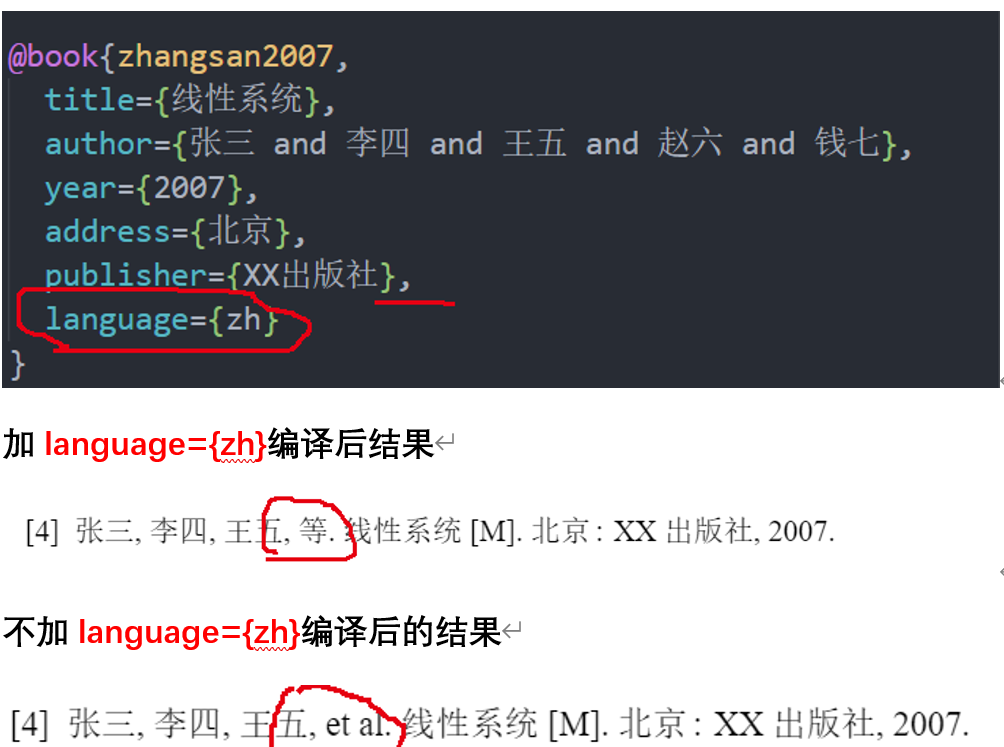
\includegraphics[width=1\textwidth]{中英文文献bib编译注意事项}
  \caption{中英文文献bib编译注意事项以作者超过3个为例进行说明}
  \label{fig_bib0}
\end{figure}


\subsection{文中参考文献的插入说明}
参考文献有两种格式引入\verb+\cite{}+以及\verb+\citep{}+。使用效果可见下面介绍:\\
1.插入会议inproceedings\cite{zhao2015bearing0}\\
2.插入教材课本book\cite{williams1991probability,chengzhaolin2006,zhangsan2007}\\
3.插入期刊article\cite{cao2011formation,xue2015formation}\\
4.插入硕博论文thesis\cite{lisi2015,wangwu2015,deans2005bearings}\\
5.插入网站misc\cite{irdawebsite,h7n9,wikipedia_moores_law}\\
6.插入专利patent\cite{xiao2012yi,p6915001}\\
7.插入新闻news报纸newspaper\cite{zhang2000,renminribao}\\
8.插入标准standard\cite{gbt3469-1983}

\textcolor{red}{注意1:参考文献格式不正确可能导致编译不通过,大家可以参考本工程中reference.bib中文献格式对网上下载不规范的bibtex文件进行修改。此外,如果上述类型里面条目有缺失会会导致编译不能输出正确格式。}

关于参考文献不同类型的进一步详细的说明可参考网站\url{https://github.com/Haixing-Hu/GBT7714-2005-BibTeX-Style}
里面的测试模板。

\subsection{参考文献的查找与引用}
多智能体系统\citep{cao2011formation}。
可以通过百度学术搜索查找参考文献(如图\ref{fig_search0}),
 \begin{figure}[!htb]
  \centering
  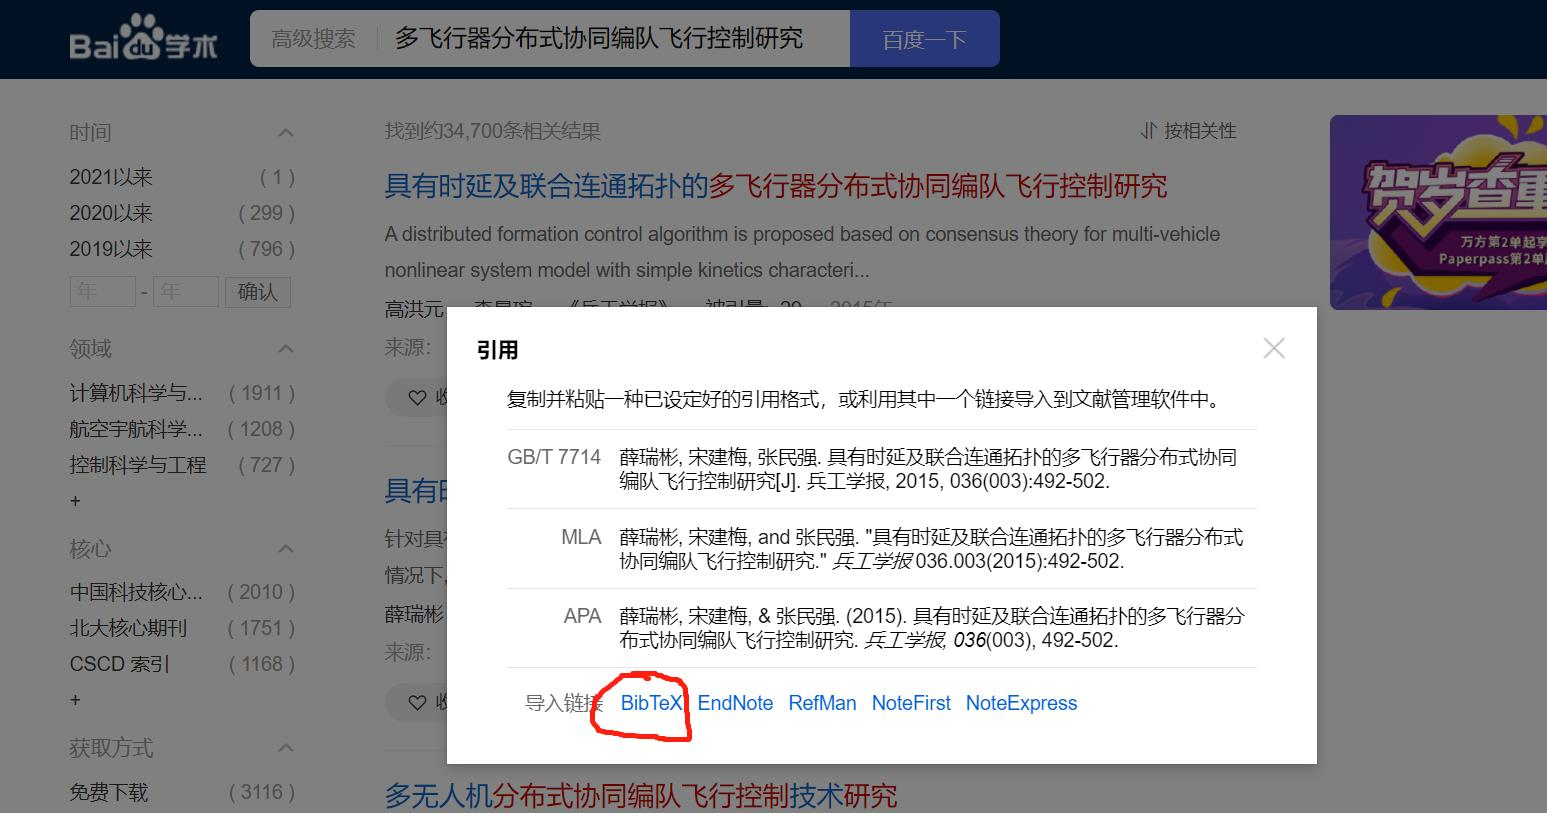
\includegraphics[width=1\textwidth]{文献搜索说明0}
  \caption{参考文献的百度学术搜索.}
  \label{fig_search0}
\end{figure}
点击bibtex,然后复制到目录文件夹中的bib文件(如图\ref{fig_search1})。此时可以调用指令为\citep{薛瑞彬2015具有时延及联合连通拓扑的多飞行器分布式协同编队飞行控制研究}。但是此时标签太长,可以适当修改标签再引用,例如把bib中的标签(第一行)的``薛瑞彬2015具有时延及联合连通拓扑的多飞行器分布式协同编队飞行控制研究"改成``xue2015formation",指令为\verb+\cite{xue2015formation}+,效果为\cite{xue2015formation}。如果进一步想管理参考文献,可新建几个bib文件并用\verb+\bibliography{en_ref,cn_ref,...}+完成。
 \begin{figure}[!htb]
  \centering
  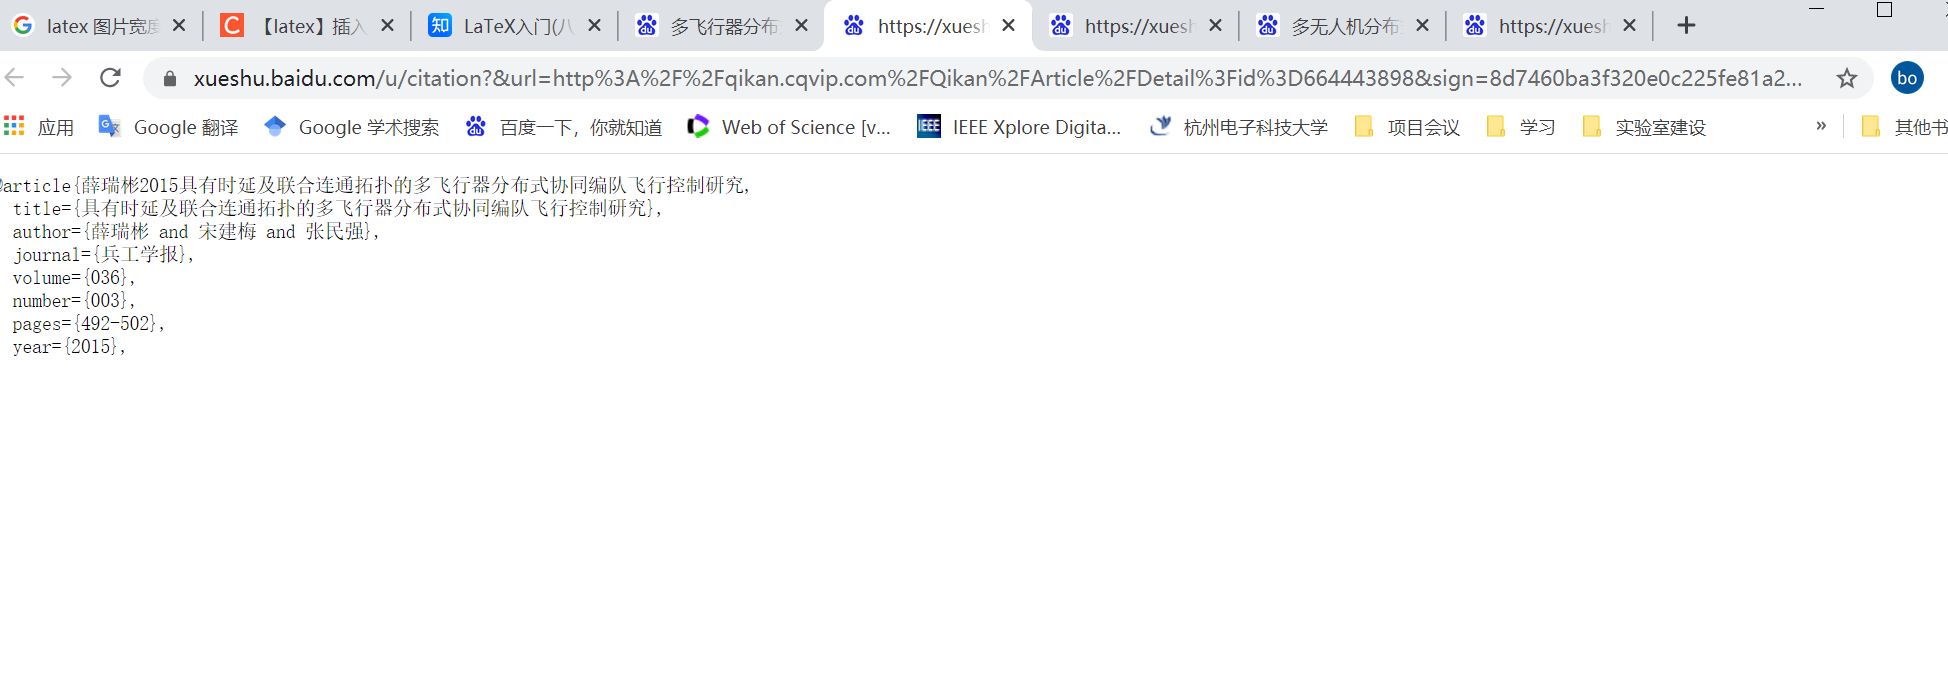
\includegraphics[width=1\textwidth]{文献搜索说明1}
  \caption{参考文献复制到bib文件.}
  \label{fig_search1}
\end{figure}

\section{插入表格}

\begin{table}[h]
    \caption{工作进度安排}
  \centering
  \setlength{\tabcolsep}{12mm}{
  \begin{tabular}{|c|c|c|}
  \hline
  序号 & 时间                  & 内容      \\ \hline
  1  & 20xx.1.8-20xx.1.12  & xxx     \\ \hline
  2  & 20xx.3.12-20xx.3.18 & xxx   \\ \hline
  \end{tabular}}
  \label{gra_process}
  \end{table}

 




%%%%%%%%%%%%%%%%%%%%%%%%%%%%%%%参考文献%%%%%%%%%%%%%%%%%%%%%%%%%%  
\myreference
\wbibliography{refs/reference}
%%%%%%%%%%%%%%%%%%%%%%%%%%%%%%%%%%%%%%%%%%%%%%%%%%%%%%%%%%%%%%%%

%%%%%%%%%%%%%%%%%%%%%%%%%%%%附录%%%%%%%%%%%%%%%%%%%%%%%%%%%%%
\myappendix
\subsection{成果}
%%%%%%%%%%%%%%%%%%%%%%%%%%%%%%%%%%%%%%%%%%%%%%%%%%%%%%%%%%%%%%%






\end{document}